%%%% fatec-article.tex, 2024/03/10

%% Classe de documento
\documentclass[
  a4paper,%% Tamanho de papel: a4paper, letterpaper (^), etc.
  12pt,%% Tamanho de fonte: 10pt (^), 11pt, 12pt, etc.
  english,%% Idioma secundário (penúltimo) (>)
  brazilian,%% Idioma primário (último) (>)
]{article}

%% Pacotes utilizados
\usepackage[]{fatec-article}
\Author{1}{Name={Mathais, Davi}}

\Author{2}{Name={\{ davi.almeida3@fatec.sp.gov.br \}}}

%% Definição das palavras-chaves/keywords
\Keyword{1}{Acidente Vascular Cerebral (AVC)}{Stroke}
\Keyword{2}{Fibrilação Atrial}{Atrial Fibrillation}
\Keyword{3}{Monitoramento Cardíaco}{Cardiac Monitoring}

%%%% Resumo no idioma primário (brazilian)
\begin{Abstract}[brazilian]%% Idioma (brazilian ou english)
  O Acidente Vascular Cerebral (AVC) isquêmico representa uma das principais causas de mortalidade e incapacidade em idosos, sendo frequentemente desencadeado por distúrbios cardíacos como arritmias e, em especial, a Fibrilação Atrial. Estudos apontam que essa condição aumenta em até cinco vezes o risco de ocorrência de AVC, devido à formação de coágulos resultantes da contração irregular do coração. A identificação precoce de alterações hemodinâmicas durante o sono é, portanto, um fator determinante para a prevenção de eventos cerebrovasculares. Diante desse contexto, este projeto propõe o desenvolvimento de um sistema inteligente de monitoramento do sono voltado à prevenção de AVC em idosos com risco cardiovascular. O dispositivo realiza a captação contínua da frequência e do ritmo cardíaco, possibilitando a análise de variações indicativas de possíveis anomalias, como episódios de arritmia. As informações coletadas são processadas e disponibilizadas em uma plataforma digital que visa auxiliar o acompanhamento médico, permitindo uma avaliação mais precisa do comportamento cardíaco noturno e fornecendo subsídios para intervenções preventivas. A proposta busca, assim, contribuir para a redução da incidência de AVC em populações vulneráveis, integrando tecnologias de monitoramento fisiológico e análise de dados a estratégias de cuidado preventivo.
\end{Abstract}

%%%% Resumo no idioma secundário (english)
\begin{Abstract}[english]%% Idioma (brazilian ou english)
The ischemic Stroke (IS) represents one of the main causes of mortality and disability among the elderly and is often triggered by cardiac disorders such as arrhythmias, particularly Atrial Fibrillation. Studies indicate that this condition increases the risk of stroke by up to five times due to the formation of blood clots resulting from the irregular contraction of the heart. Early identification of hemodynamic changes during sleep is, therefore, a determining factor in preventing cerebrovascular events. In this context, this project proposes the development of an intelligent sleep monitoring system aimed at preventing strokes in elderly individuals with cardiovascular risk. The device continuously records heart rate and rhythm, allowing the analysis of variations indicative of possible anomalies, such as arrhythmia episodes. The collected information is processed and made available on a digital platform designed to support medical monitoring, enabling a more accurate assessment of nocturnal cardiac behavior and providing data for preventive interventions. The proposal thus seeks to contribute to reducing the incidence of strokes in vulnerable populations by integrating physiological monitoring technologies and data analysis into preventive care strategies.
\end{Abstract}

%% Processamento de entradas (itens) do índice remissivo (makeindex)
\makeindex%

%% Arquivo(s) de referências
\addbibresource{fatec-article.bib}

%% Início do documento
\begin{document}

% Seções e subseções
%\section{Título de Seção Primária}%

%\subsection{Título de Seção Secundária}%

%\subsubsection{Título de Seção Terciária}%

%\paragraph{Título de seção quaternária}%

%\subparagraph{Título de seção quinária}%

\section*{Introdução}%
\label{sect:intro}
O Acidente Vascular Cerebral (AVC) é uma das principais causas de mortalidade e incapacidade no mundo, representando um desafio crescente para os sistemas de saúde pública e para a qualidade de vida da população idosa. Segundo a Organização Mundial da Saúde (OMS), cerca de 15 milhões de pessoas sofrem um AVC a cada ano, sendo que um terço evolui para óbito e outro terço apresenta sequelas permanentes \parencite{WHO2023}. No Brasil, o AVC é a segunda principal causa de morte, com incidência especialmente elevada entre indivíduos com mais de 60 anos, faixa etária em que doenças cardiovasculares e distúrbios do ritmo cardíaco tornam-se mais frequentes \parencite{MinisterioSaude2022}.

O AVC pode ser classificado em dois tipos principais: hemorrágico e isquêmico. O tipo isquêmico, responsável por aproximadamente 85\% dos casos, ocorre quando há obstrução do fluxo sanguíneo cerebral devido à formação de coágulos, frequentemente relacionados a arritmias como a Fibrilação Atrial (FA) \parencite{JAMAAtrialFib,WJGNetStrokeRisk}. 

A Fibrilação Atrial é caracterizada por uma ativação elétrica atrial caótica, rápida e desorganizada. Em um ritmo cardíaco normal (sinusal), o Eletrocardiograma (ECG) exibe uma onda P clara antes de cada batimento, representando a contração unificada dos átrios. Na FA, essa atividade elétrica unificada desaparece; a onda P é substituída por ondas fibrilatórias irregulares (conhecidas como "ondas f"). Isso significa que os átrios deixam de contrair de forma eficaz e passam a apenas "tremular" ou "fibrilar".

Essa perda da contração atrial efetiva leva a um estado de estase sanguínea — uma lentidão significativa do fluxo de sangue — especialmente em uma pequena bolsa do átrio esquerdo chamada apêndice atrial esquerdo. Esse sangue "parado" tem alta propensão a formar trombos (coágulos sanguíneos). Quando um desses trombos se desprende, ele viaja pela artéria aorta até o cérebro, causando uma embolia cerebral e, consequentemente, o AVC isquêmico. Assim, o reconhecimento precoce de irregularidades no ritmo cardíaco é um fator decisivo para reduzir a incidência e a gravidade dos eventos cerebrovasculares \parencite{PubMedSAFARIS}.

Estudos apontam que alterações cardíacas sutis, muitas vezes assintomáticas, tendem a se manifestar durante o sono, quando o corpo entra em um estado de repouso e autorregulação fisiológica \parencite{SnifBrasil2023,JMIRContactless2024}. Nesse contexto, o monitoramento contínuo dos sinais vitais noturnos surge como uma ferramenta essencial para a vigilância clínica de idosos com risco cardiovascular elevado, especialmente aqueles que vivem sozinhos ou possuem histórico de doenças cardíacas.

Com os avanços recentes em sensores biomédicos e Internet das Coisas (IoT), tornou-se possível desenvolver dispositivos capazes de capturar e transmitir dados fisiológicos em tempo real, oferecendo suporte ao acompanhamento médico remoto \parencite{Ansys2022}. No entanto, o verdadeiro potencial dessas tecnologias está em sua integração ao trabalho médico, ampliando a capacidade de diagnóstico e prevenção por meio de informações precisas e continuamente atualizadas.

Diante dessa perspectiva, o presente projeto propõe o desenvolvimento de um sistema inteligente de monitoramento de sono voltado à prevenção de AVC em idosos, cujo foco central está tanto na captação e análise de sinais vitais durante o sono, quanto na disponibilização dessas informações ao profissional de saúde. O sistema busca fornecer ao médico um panorama detalhado do comportamento cardíaco noturno do paciente, permitindo identificar precocemente padrões de risco e embasar decisões clínicas de prevenção e tratamento. Dessa forma, pretende-se unir inovação tecnológica e relevância médica em uma solução que promova um cuidado mais humanizado, contínuo e baseado em evidências.

Além de seu caráter científico e tecnológico, o projeto também se insere no âmbito das ações de extensão universitária, em consonância com as diretrizes do Fórum de Pró-Reitores de Extensão das Instituições Públicas de Educação Superior Brasileiras (FORPROEX). Nesse contexto, contempla as áreas temáticas de Saúde e Tecnologia e Produção, e está alinhado às linhas de extensão de Desenvolvimento Tecnológico e Saúde Humana, por promover a criação de uma solução inovadora voltada à prevenção de AVC em idosos. Essa integração entre conhecimento científico, inovação e responsabilidade social reforça o compromisso da instituição com a formação cidadã e com o impacto positivo das tecnologias na melhoria da qualidade de vida da população.

\begin{center}
\captionof{figure}{Exemplo de ondas P no ECG}
\label{fig:introducao-exemplo}
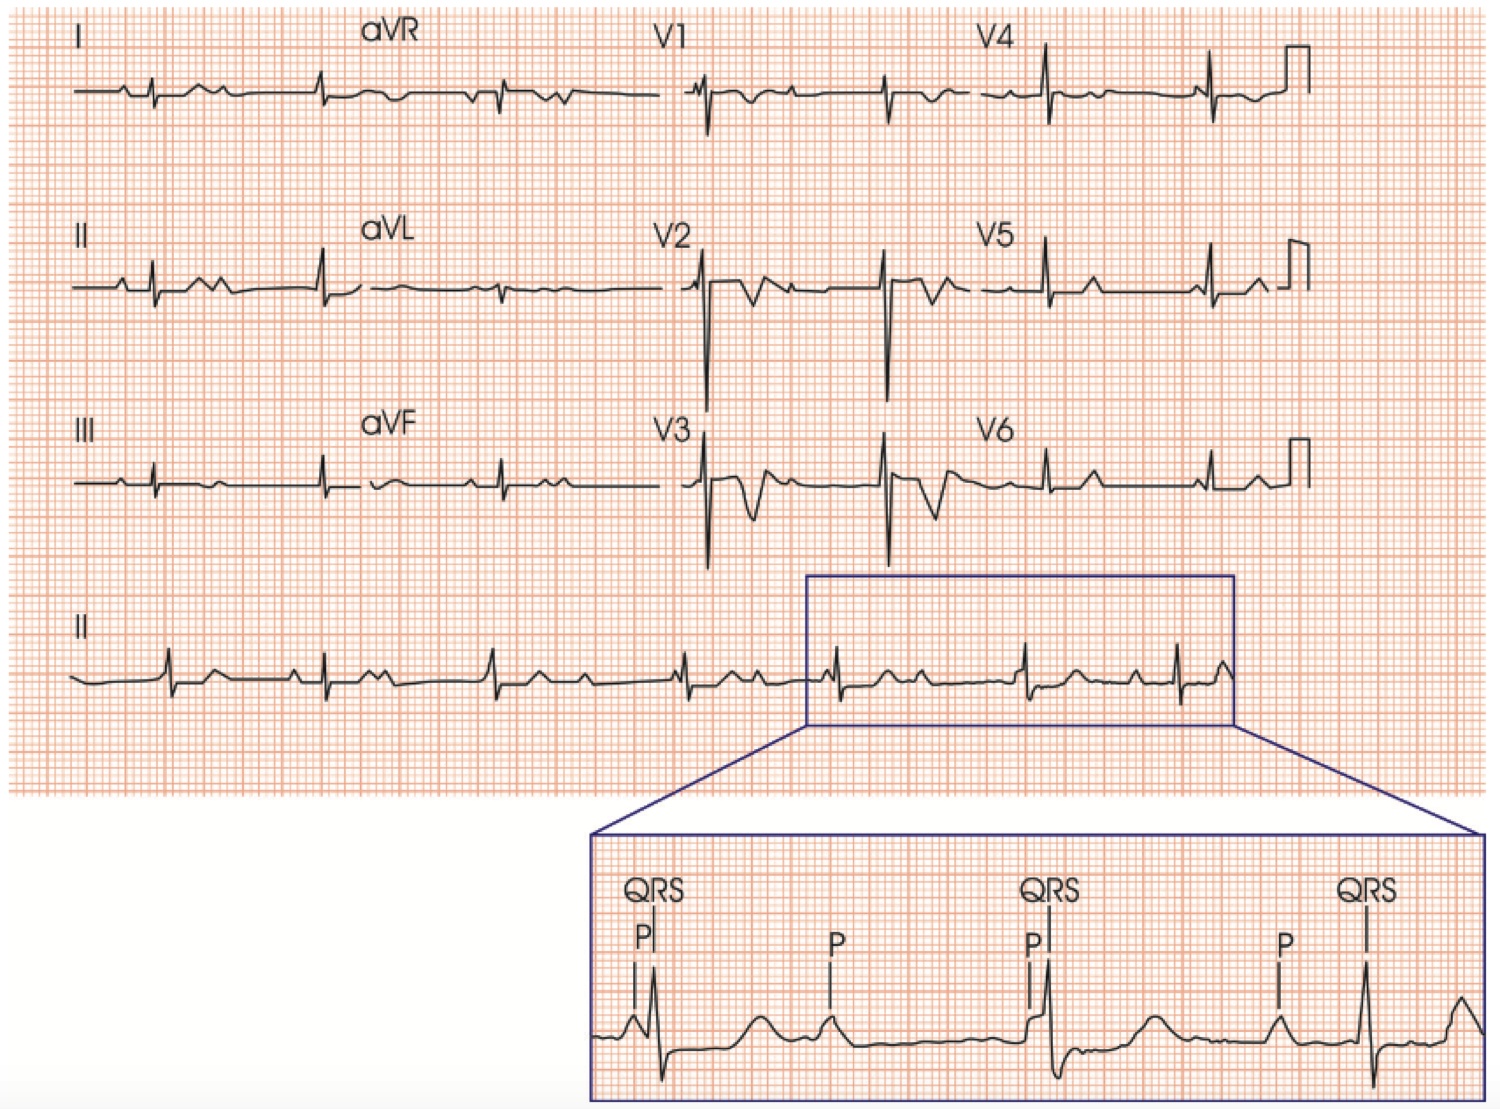
\includegraphics[width=0.8\textwidth]{Illustrations/ondas-p.png}
\vspace{1em}
\SourceOrNote{Adaptado de \textcite{PortalAfya2025}}
\end{center}

\begin{center}
\captionof{figure}{Exemplo de ondas f no ECG}
\label{fig:introducao-exemplo2}
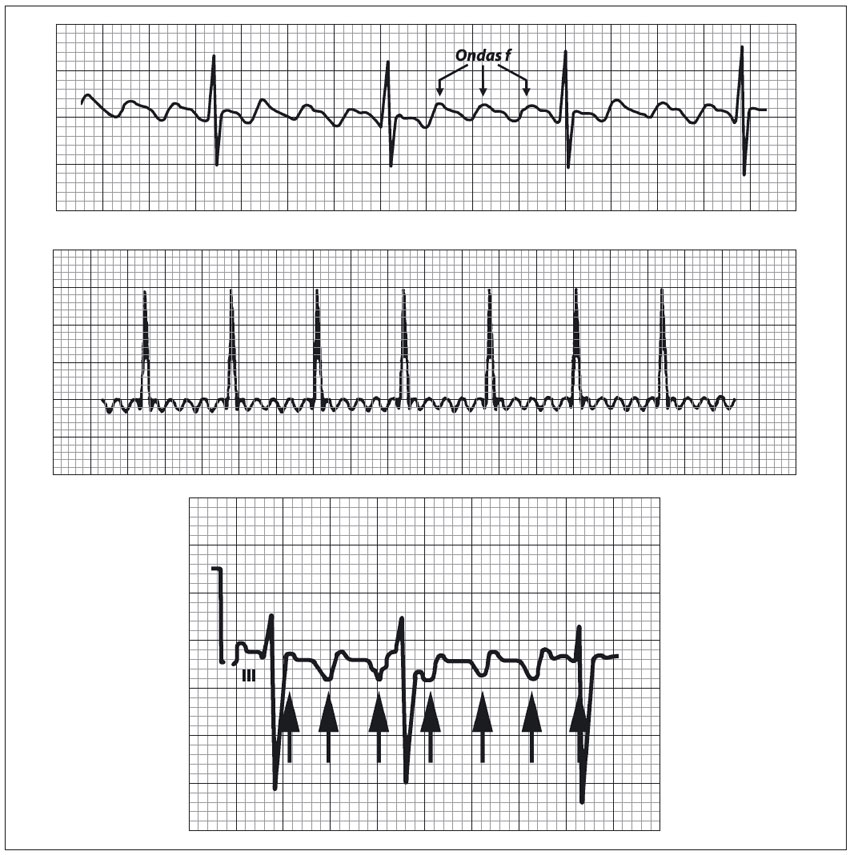
\includegraphics[width=0.7\textwidth]{Illustrations/ondas-f.jpg}
\vspace{1em}
\SourceOrNote{Adaptado de \textcite{PortalAfya2025}}
\end{center}


\section*{OBJETIVO} \label{sect:obj}

O presente projeto tem como objetivo geral o desenvolvimento de um sistema inteligente de monitoramento de sono voltado à prevenção de Acidente Vascular Cerebral (AVC) isquêmico em idosos com risco cardiovascular elevado. O sistema visa realizar a coleta, análise e disponibilização contínua de sinais vitais, com ênfase na frequência e ritmo cardíaco durante o período de repouso, a fim de possibilitar o acompanhamento médico preciso e preventivo.\\

Como objetivos específicos, destacam-se:\\

\begin{enumerate}[itemsep=1em]
    \item Desenvolver um dispositivo de monitoramento contínuo capaz de captar sinais vitais de forma não invasiva e precisa durante o sono;
    \item Registrar, armazenar e organizar os dados coletados em um ambiente seguro, possibilitando o acompanhamento longitudinal da saúde do paciente;
    \item Processar e analisar os dados para identificar variações significativas ou padrões que possam indicar risco de arritmias cardíacas associadas ao AVC isquêmico;
    \item Disponibilizar os resultados de forma acessível e interpretável ao profissional de saúde, fornecendo suporte à tomada de decisões clínicas relacionadas à prevenção e intervenção precoce;
    \item Contribuir para a redução da incidência e mortalidade associadas ao AVC, promovendo um modelo de cuidado mais contínuo, tecnológico e centrado na prevenção.\\
\end{enumerate}

Dessa forma, o projeto busca integrar tecnologia, ciência de dados e prática médica, oferecendo ao profissional de saúde uma ferramenta capaz de otimizar o diagnóstico preventivo e aperfeiçoar o processo decisório clínico. A interpretação automatizada e a disponibilização visual dos dados ampliam a capacidade do médico em identificar riscos de forma antecipada, impactando diretamente na qualidade de vida e na sobrevida dos pacientes idosos.

\section*{ESTADO DA ARTE} \label{sect:estadoarte}

Nas últimas décadas, o monitoramento remoto de sinais vitais tem se consolidado como uma das vertentes mais promissoras da tecnologia aplicada à saúde, especialmente no contexto da medicina preventiva e do envelhecimento populacional. O avanço dos sensores ópticos, da Internet das Coisas (IoT) e da Inteligência Artificial permitiu o desenvolvimento de sistemas capazes de captar e interpretar dados fisiológicos em tempo real, possibilitando a identificação precoce de anomalias cardíacas associadas a eventos cerebrovasculares, como o Acidente Vascular Cerebral (AVC) isquêmico.

Entre as abordagens mais promissoras para o monitoramento contínuo da frequência e do ritmo cardíaco destaca-se a fotopletismografia (PPG), uma técnica óptica não invasiva que mensura variações no volume sanguíneo por meio da luz refletida ou transmitida pelos tecidos biológicos. Essa metodologia tem se mostrado altamente eficaz na detecção precoce de arritmias, em especial da fibrilação atrial (FA). O estudo conduzido por \textcite{Lubitz2022}, publicado na revista Circulation, avaliou a aplicação de algoritmos de detecção de FA baseados em PPG, demonstrando elevada sensibilidade e especificidade na identificação de eventos arrítmicos por meio de dispositivos vestíveis. Os resultados evidenciaram o potencial clínico dessa tecnologia para o rastreamento contínuo e não supervisionado de distúrbios cardíacos, reforçando sua relevância em estratégias de prevenção secundária de AVC e na promoção de uma vigilância cardíaca remota e acessível.

Apesar da precisão obtida com a fotopletismografia, a interpretação manual dos sinais ainda representa um desafio clínico devido ao grande volume de dados gerados. Nesse cenário, o avanço de técnicas de aprendizado profundo baseadas em Inteligência Artificial surge como resposta ao desafio da análise automatizada e em tempo real desses sinais. Pesquisas recentes, como a de \textcite{Charlton2023}, demonstram que o emprego de redes neurais profundas na interpretação de sinais fotopletismográficos possibilita a detecção em tempo real de anomalias cardíacas e respiratórias com elevada acurácia, mesmo em ambientes domésticos. Essa capacidade de processamento dinâmico permite identificar padrões sutis e preditivos, viabilizando um rastreamento proativo de eventos cardiovasculares.

Em paralelo, o estudo conduzido por \textcite{DeVries2023} reforça a confiabilidade dos dispositivos vestíveis na aquisição contínua de dados de sono e frequência cardíaca em contextos não controlados, validando sua aplicabilidade clínica. A sinergia entre inteligência artificial e biossensoriamento representa, portanto, um avanço significativo rumo à assistência médica preventiva e personalizada, em que o monitoramento remoto fornece subsídios objetivos para tomadas de decisão clínicas baseadas em dados.

Contudo, apesar dos avanços, observa-se que a maioria das soluções existentes tem foco na automonitorização pelo próprio paciente, sem uma integração direta com o profissional de saúde responsável pelo acompanhamento clínico. Nesse contexto, o projeto proposto neste trabalho diferencia-se ao centralizar o médico como principal usuário final do sistema, oferecendo uma plataforma de apoio à interpretação diagnóstica e à tomada de decisão terapêutica, transformando dados de sinais vitais em informações clínicas de alto valor preditivo.

A proposta, portanto, alinha-se às tendências mais recentes de telemonitoramento e medicina personalizada, mas introduz um enfoque inovador ao unir o monitoramento contínuo do sono, a análise inteligente de anomalias cardíacas e o suporte direto à decisão médica, com o objetivo de aprimorar a prevenção de AVC em idosos e reduzir a mortalidade associada a eventos cerebrovasculares.

\section*{METODOLOGIA} \label{sect:metodologia}

O presente estudo adota uma abordagem experimental e descritiva, centrada no desenvolvimento e validação inicial de um sistema de monitoramento inteligente de sono para prevenção de Acidente Vascular Cerebral (AVC) em idosos. O foco principal está no monitoramento contínuo de sinais vitais durante o sono, aliado à interpretação automatizada dos dados clínicos, de modo a fornecer subsídios para a tomada de decisão médica.

A metodologia foi estruturada em quatro etapas principais: Aquisição dos sinais fisiológicos, transmissão e armazenamento dos dados, análise e processamento inteligente e visualização e interpretação médica.\\

\begin{figure}[!htb]
\centering
\caption{Visão geral do sistema}
\label{fig:metodologia-sistema}
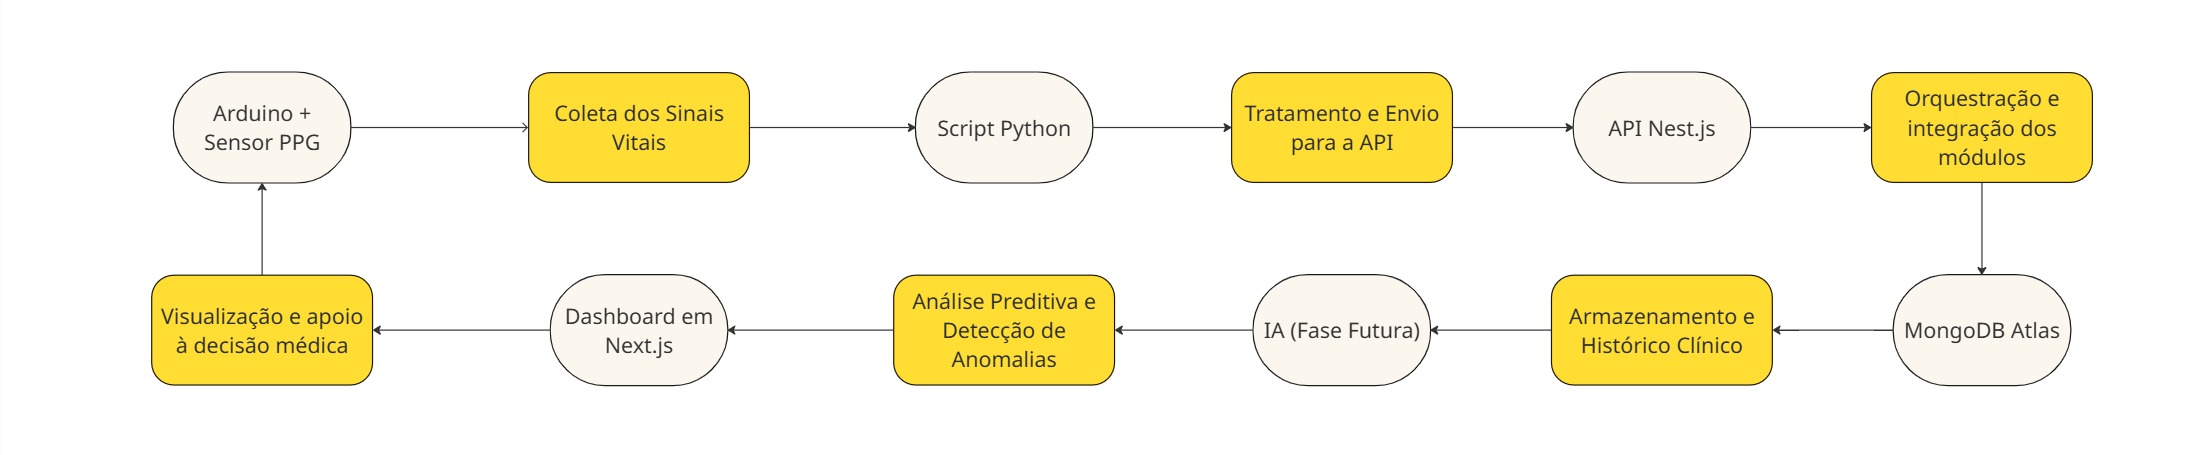
\includegraphics[width=0.8\textwidth]{Illustrations/Fluxograma.jpg}\\
\SourceOrNote{Autoria Própria (2025)}
\end{figure}

\subsection*{Aquisição dos sinais fisiológicos}

Na primeira etapa, foi utilizado um sensor de pulso cardíaco óptico acoplado a uma plataforma Arduino, responsável pela coleta contínua dos sinais de frequência e ritmo cardíaco. O sensor baseia-se no princípio da fotopletismografia (PPG), técnica óptica não invasiva que mensura variações do volume sanguíneo a partir da luz refletida pelos tecidos biológicos \parencite{TimarFulepPPG,Charlton2023}. Durante os testes laboratoriais, o dispositivo foi posicionado na extremidade do dedo do participante, possibilitando a captação precisa e ininterrupta dos batimentos por minuto (BPM) e do padrão rítmico do pulso durante o período de sono.

\subsection*{Transmissão e armazenamento dos dados}

Os dados captados pelo Arduino são transmitidos via interface serial para um computador intermediário, responsável por atuar como ponte entre o dispositivo físico e a infraestrutura de armazenamento. Nessa etapa, as informações são processadas por um script desenvolvido em Python, que executa funções de leitura contínua, filtragem de ruídos e normalização dos valores obtidos. O script também realiza a padronização temporal das amostras, garantindo a consistência das séries de dados ao longo das sessões de monitoramento.

Após a validação, os dados são estruturados em formato JSON (JavaScript Object Notation) e enviados via requisições HTTP para o servidor, onde são armazenados em um banco de dados não relacional MongoDB, hospedado em um cluster do MongoDB Atlas. Essa configuração em nuvem assegura alta disponibilidade, escalabilidade horizontal e redundância geográfica, características essenciais para sistemas de monitoramento contínuo e com potencial expansão para múltiplos usuários.

Essa estrutura de armazenamento fornece suporte robusto para futuras correlações clínicas entre variáveis fisiológicas e risco de AVC, além de servir como base de treinamento para os modelos de Inteligência Artificial planejados. A integração entre o script em Python e o banco MongoDB garante eficiência na comunicação, redução de perdas de pacotes de dados e segurança no tratamento das informações biomédicas, consolidando a arquitetura como uma fundação confiável para análises médicas baseadas em dados.

\subsection*{Orquestração e integração via API}

A comunicação entre os módulos do sistema é realizada por meio de uma API desenvolvida em Nest.js, que atua como camada de orquestração central da aplicação. Essa API é responsável por receber os dados processados em Python, armazená-los no banco MongoDB, e disponibilizá-los de forma segura e estruturada para os módulos de visualização e análise.
Além disso, a arquitetura da API segue princípios de modularidade e desacoplamento, garantindo a expansão futura para novos serviços, como a integração com modelos de IA e dashboards personalizados para diferentes perfis de usuários (médicos, cuidadores e pesquisadores). A adoção de protocolos RESTful e autenticação via tokens JWT assegura confiabilidade, segurança e rastreabilidade em todo o fluxo de dados biomédicos.

\subsection*{Análise e processamento inteligente}

Atualmente em estágio de planejamento e experimentação laboratorial, o módulo de Inteligência Artificial (IA) constitui o núcleo analítico do sistema proposto, sendo responsável por interpretar os dados biomédicos armazenados e detectar padrões anômalos relacionados à frequência e ao ritmo cardíaco. O principal objetivo dessa camada é identificar episódios de Fibrilação Atrial (FA) — um dos principais precursores de AVC isquêmico — por meio da análise de séries temporais obtidas a partir de sinais fotopletismográficos (PPG).

O desenvolvimento do módulo baseia-se na aplicação de técnicas de aprendizado supervisionado e modelos de redes neurais convolucionais (CNNs) adaptados para o tratamento de dados fisiológicos contínuos. As CNNs são particularmente adequadas para essa tarefa por sua capacidade de extrair características locais e padrões rítmicos sutis dos sinais temporais, permitindo a diferenciação entre oscilações cardíacas regulares e irregularidades compatíveis com episódios arrítmicos. Estão sendo estudadas abordagens híbridas que combinam CNNs com redes recorrentes (RNNs) ou Long Short-Term Memory (LSTM), de forma a ampliar a capacidade do modelo em capturar dependências de longo prazo presentes nas variações cardíacas noturnas.

Os resultados obtidos pela IA serão retroalimentados ao banco de dados principal, vinculados a cada paciente de forma segura e anonimizada. Essa retroalimentação permitirá a construção de um histórico clínico longitudinal, no qual cada nova análise complementa as anteriores, formando um ecossistema de aprendizado contínuo. Paralelamente, os insights gerados pelo modelo — como alertas de risco ou padrões anômalos — serão disponibilizados ao médico por meio da API central em Nest.js, que orquestra a comunicação entre os módulos de armazenamento, análise e interface visual.

No futuro, essa camada analítica permitirá a evolução do sistema de uma abordagem meramente descritiva para uma interpretação preditiva, capaz de emitir alertas automatizados em tempo quase real e oferecer apoio à decisão clínica baseada em dados. Essa integração entre IA e prática médica não apenas aprimora a precisão diagnóstica, como também potencializa a prevenção de eventos cerebrovasculares em populações de risco, consolidando o sistema como uma ferramenta de suporte clínico inteligente e escalável.

\subsection*{Visualização e interpretação médica}

A camada de visualização foi desenvolvida utilizando o framework Next.js, constituindo um dashboard clínico interativo projetado para a interpretação e acompanhamento de dados fisiológicos de pacientes idosos em monitoramento. Essa interface atua como elo direto entre os módulos tecnológicos do sistema e o profissional de saúde, transformando dados técnicos em informações clínicas de alto valor interpretativo.

O painel é composto por gráficos dinâmicos e indicadores em tempo quase real, que exibem tanto os dados brutos dos sinais vitais — como frequência cardíaca, ritmo e variação temporal — quanto as interpretações analíticas geradas automaticamente pela camada de Inteligência Artificial. Esses resultados são organizados de forma hierarquizada, permitindo ao médico alternar entre visualizações macro, que mostram tendências de longo prazo, e análises detalhadas, que possibilitam a identificação de anomalias pontuais durante o período de sono.

A arquitetura do dashboard foi estruturada com foco em usabilidade, clareza visual e precisão na comunicação dos dados clínicos, utilizando princípios de design centrado no usuário médico. Essa abordagem visa reduzir a carga cognitiva durante a análise, oferecendo recursos como filtros temporais, comparativos históricos, alertas visuais e resumos interpretativos. Dessa forma, o sistema facilita a interpretação contextualizada das informações, promovendo uma tomada de decisão mais fundamentada e eficiente.

A comunicação entre a interface e os demais módulos é orquestrada pela API central desenvolvida em Nest.js, responsável por mediar as requisições entre o banco de dados MongoDB Atlas, os scripts de processamento em Python e o módulo de IA. Essa arquitetura modular e desacoplada garante baixa latência nas consultas, consistência dos dados apresentados e alta disponibilidade do sistema, permitindo que as informações clínicas sejam acessadas com segurança e confiabilidade.

O protótipo resultante integra, de maneira coesa, todos os componentes tecnológicos do projeto — o módulo físico de captação (Arduino), o processamento de dados (Python), a API de orquestração (Nest.js), o banco em nuvem (MongoDB Atlas) e a interface médica (Next.js). Essa sinergia entre hardware, backend, infraestrutura em nuvem e inteligência artificial confere ao sistema robustez, escalabilidade e eficiência operacional, assegurando a precisão na análise dos sinais vitais e ampliando o potencial clínico do monitoramento remoto como ferramenta de apoio à prevenção de AVC em idosos.

Além disso, o dashboard não se limita a uma visualização estática, mas propõe uma plataforma dinâmica de suporte à decisão médica, em que a combinação de dados históricos, análises preditivas e alertas automáticos cria um ambiente propício à medicina personalizada e baseada em dados. Com isso, o sistema consolida-se como uma ferramenta inovadora voltada à vigilância cardíaca remota, contribuindo para a redução da mortalidade e das sequelas associadas a eventos cerebrovasculares.

\section*{RESULTADOS PRELIMINARES}\label{sect:resultados}

Até o momento, o projeto alcançou resultados relevantes, destacando-se o desenvolvimento de um protótipo funcional do sistema de monitoramento inteligente de sono, a validação experimental em ambiente laboratorial e a implementação dos módulos de coleta, armazenamento e visualização dos dados fisiológicos. Os testes realizados confirmaram a viabilidade técnica do sistema, demonstrando coerência nos sinais captados e estabilidade na comunicação entre o Arduino e a aplicação de backend.

\subsection*{Coleta e estabilidade dos sinais}

Durante os testes, o sensor óptico de fotopletismografia (PPG), acoplado ao Arduino, apresentou resposta estável e contínua na leitura dos batimentos cardíacos. Esse resultado confirma a viabilidade do uso do sensor em aplicações de monitoramento não invasivo, desde que o dispositivo esteja adequadamente fixado e em ambiente com baixa interferência luminosa.

Os dados coletados incluíram frequência cardíaca (BPM), padrão rítmico de pulso e nível relativo de perfusão, permitindo a análise da regularidade dos ciclos cardíacos durante o repouso. Essa base inicial de dados já fornece indícios sobre a detecção de variações de ritmo compatíveis com episódios de arritmia leve, que serão posteriormente exploradas na etapa de aplicação da Inteligência Artificial.

Entretanto, o estágio atual ainda apresenta limitações inerentes à fase inicial de prototipagem. O dispositivo permanece fisicamente conectado ao computador via cabo, o que restringe a mobilidade do usuário e inviabiliza o uso contínuo durante o sono em condições domésticas reais. Além disso, a transmissão dos dados não ocorre de forma autônoma, dependendo de um intermediário local para envio das medições ao banco de dados, o que limita a escalabilidade do sistema.

Essas restrições, no entanto, já foram consideradas na arquitetura do projeto. A versão futura prevê a integração de módulos de conectividade sem fio, como Wi-Fi ou Bluetooth Low Energy (BLE), permitindo que o dispositivo opere de forma totalmente independente e envie os dados diretamente à API, responsável por orquestrar a comunicação entre sensores, banco de dados e camada de análise.

\subsection*{Transmissão e integração dos módulos}

O script em Python foi testado com sucesso na leitura serial dos dados provenientes do Arduino, realizando a padronização e o envio para a API em Nest.js. 

Durante os testes iniciais de integração, foi possível verificar a comunicação consistente entre os módulos de coleta e armazenamento, assegurando que os dados captados pelo Arduino fossem transmitidos corretamente para a API e posteriormente, armazenados no banco de dados MongoDB Atlas. Ainda que a etapa de validação quantitativa em larga escala esteja em fase de planejamento, os resultados preliminares indicam estabilidade no fluxo de dados e funcionamento adequado das rotas RESTful, confirmando a viabilidade técnica da arquitetura proposta para monitoramento contínuo e armazenamento seguro das informações fisiológicas.

\subsection*{Visualização e interpretação dos dados}

A interface de visualização desenvolvida em Next.js apresentou excelente desempenho na renderização dos dados armazenados, permitindo a análise gráfica da frequência cardíaca e do ritmo pulsátil após cada sessão de monitoramento.

O dashboard médico foi projetado para oferecer uma visão unificada e intuitiva dos parâmetros vitais, apresentando:\\

\begin{itemize}[itemsep=0.5em]
    \item Gráficos dinâmicos de variação de BPM;
    \item Indicadores de estabilidade cardíaca;
    \item Logs de eventos anômalos;\\
\end{itemize}

Esses recursos facilitam a interpretação clínica dos dados coletados, fornecendo ao profissional de saúde subsídios objetivos para apoiar decisões baseadas em evidências. Embora a camada de Inteligência Artificial ainda não esteja implementada, a arquitetura do sistema foi planejada para permitir a integração futura de modelos preditivos no backend sem necessidade de reestruturação.

De forma geral, os resultados preliminares demonstram que o projeto é tecnicamente viável e operacionalmente estável. O desempenho do sistema no ambiente laboratorial indica alta confiabilidade na coleta e transmissão dos sinais vitais, eficiência na comunicação entre módulos e adequada responsividade da interface web.

Esses avanços estabelecem uma base sólida para a próxima etapa do projeto, que consistirá na implementação e treinamento dos modelos de IA voltados à detecção automática de anomalias cardíacas e predição de risco de AVC. Essa evolução permitirá validar o potencial do sistema como ferramenta de apoio à decisão médica, reforçando seu propósito central de atuar preventivamente na preservação da vida e na melhoria da saúde cardiovascular de idosos.

\section*{CONCLUSÃO}\label{sect:conclusao}

A presente pesquisa reafirma o papel fundamental da tecnologia como instrumento catalisador na prevenção e monitoramento de doenças cardiovasculares, especialmente no contexto do envelhecimento populacional e do risco aumentado de Acidente Vascular Cerebral (AVC). O projeto de Monitoramento Inteligente do Sono identifica uma lacuna crítica na interseção entre análise de sinais vitais e apoio à decisão clínica, propondo uma solução concreta, sustentada em fundamentos científicos sólidos e em experimentação laboratorial voltada à validação técnica do sistema.

O protótipo desenvolvido, composto por um sensor óptico de baixo custo integrado a uma infraestrutura modular baseada em API Nest.js, banco de dados MongoDB e interface em Next.js, demonstra a viabilidade de um sistema capaz de coletar e interpretar parâmetros fisiológicos com confiabilidade. Mais do que um dispositivo de monitoramento, o sistema se configura como uma ferramenta de suporte médico, oferecendo dados clínicos objetivos que podem subsidiar a tomada de decisões preventivas e terapêuticas voltadas à redução da incidência de AVC em idosos.

Importa destacar que o projeto não se propõe a substituir o acompanhamento médico tradicional, mas a complementá-lo, promovendo uma integração inteligente entre tecnologia e prática clínica. Essa convergência potencializa o diagnóstico precoce, amplia a eficiência da vigilância de pacientes de risco e reforça o papel do profissional de saúde como agente central na interpretação dos dados. Assim, o sistema contribui para a consolidação de um modelo de medicina mais preditiva, personalizada e orientada por dados.

Entre as perspectivas futuras, destaca-se a transição do protótipo com conexão física via fio para uma versão totalmente sem fio, visando maior conforto e aplicabilidade no ambiente doméstico. Também se prevê a integração de algoritmos de Inteligência Artificial capazes de identificar padrões fisiológicos indicativos de risco de AVC, bem como a ampliação da base de dados para treinamento e validação desses modelos. Em paralelo, pretende-se aprimorar a interface de visualização e os relatórios médicos, garantindo maior precisão e usabilidade no acompanhamento clínico remoto.

Dessa forma, o Monitoramento Inteligente do Sono transcende sua dimensão técnica e assume um papel estratégico na promoção da saúde, longevidade e qualidade de vida da população idosa, ao alinhar inovação tecnológica, rigor científico e responsabilidade social. O projeto consolida-se, assim, como uma contribuição significativa para o avanço da medicina preventiva e para o fortalecimento das práticas de cuidado baseadas em evidências e conectividade digital.

Adicionalmente, a iniciativa está alinhada aos Objetivos de Desenvolvimento Sustentável da ONU, em especial a ODS 3 – Saúde e Bem-Estar, ao promover soluções que visam reduzir a mortalidade por doenças cardiovasculares, garantir acesso a cuidados preventivos e apoiar a qualidade de vida de populações vulneráveis. Nesse sentido, o projeto demonstra como a convergência entre tecnologia, ciência e políticas de saúde pode contribuir para metas globais de promoção da saúde, equidade e inclusão.

\printbibliography

%% Elementos pós-textuais (opcionais): Apêndice e Anexo
%Caso for utilizar, basta retirar o símbolo de % na frente do comando
%%%%% Elementos pós-textuais
%%
%% Glossário, apêndices, anexos e índice remissivo (opcionais).

%% Apêndices
\begin{Appendix}

\section{Título de Apêndice}%
\label{sect:apx-a1}

Exemplo de apêndice (\Cref{sect:apx-a1}) em uma seção de \nameref{sect:appendix}.

\subsection{Título de Seção Secundária de Apêndice}%
\label{ssect:apx-a2}

Exemplo de seção secundária de apêndice (\Cref{ssect:apx-a2}).

\subsubsection{Título de Seção Terciária de Apêndice}%
\label{sssect:apx-a3}

Exemplo de seção terciária de apêndice (\Cref{sssect:apx-a3}).

\paragraph{Título de seção quaternária de Apêndice}%
\label{prgh:apx-a4}

Exemplo de seção quaternária de apêndice (\Cref{prgh:apx-a4}).

\subparagraph{Título de seção quinária de Apêndice}%
\label{sprgh:apx-a5}

Exemplo de seção quinária de apêndice (\Cref{sprgh:apx-a5}).

\end{Appendix}

%% Anexos
\begin{Annex}

\section{Título de Anexo}%
\label{sect:anx-a1}

Exemplo de anexo (\Cref{sect:anx-a1}) em uma seção de \nameref{sect:annex}.

\subsection{Título de Seção Secundária de Anexo}%
\label{ssect:anx-a2}

Exemplo de seção secundária de anexo (\Cref{ssect:anx-a2}).

\subsubsection{Título de Seção Terciária de Anexo}%
\label{sssect:anx-a3}

Exemplo de seção terciária de anexo (\Cref{sssect:anx-a3}).

\paragraph{Título de seção quaternária de Anexo}%
\label{prgh:anx-a4}

Exemplo de seção quaternária de anexo (\Cref{prgh:anx-a4}).

\subparagraph{Título de seção quinária de Anexo}%
\label{sprgh:anx-a5}

Exemplo de seção quinária de anexo (\Cref{sprgh:anx-a5}).

\end{Annex}

%% Índice remissivo
\printindex%


%% Fim do documento
\end{document}